\documentclass[12pt,titlepage]{article}

\usepackage{graphics}
\usepackage{pdflscape}
\usepackage{array}
\usepackage{color}
\usepackage{colortbl}
\usepackage{xcolor}
\usepackage{url,amsfonts,epsfig}
\usepackage[applemac]{inputenc} %comando per le lettere accentate se usate mac  
%\usepackage[T1]{fontenc}
%\usepackage[utf8]{inputenc}
\usepackage[english]{babel}
%\usepackage[latin1]{inputenc} % comando per le lettere accentate se usate pc  
\usepackage[pagebackref]{hyperref}
\hypersetup{
colorlinks=false,
allbordercolors=white
}

\usepackage{listings}
\usepackage{color}

\definecolor{dkgreen}{rgb}{0,0.6,0}
\definecolor{gray}{rgb}{0.5,0.5,0.5}
\definecolor{mauve}{rgb}{0.58,0,0.82}

\lstset{frame=none,
  language=Java,
  aboveskip=3mm,
  belowskip=3mm,
  showstringspaces=false,
  columns=flexible,
  basicstyle={\small\ttfamily},
  numbers=none,
  numberstyle=\tiny\color{gray},
  keywordstyle=\color{blue},
  commentstyle=\color{dkgreen},
  stringstyle=\color{mauve},
  breaklines=true,
  breakatwhitespace=true,
  tabsize=3
}

\begin{document}
%Code for title page
\begin{titlepage}
\centering
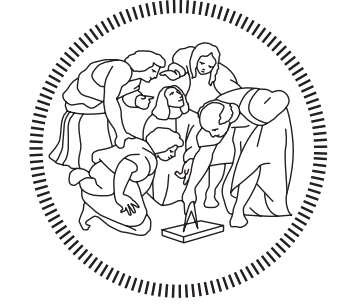
\includegraphics[width=0.4\textwidth]{Logos/LogoPolimi}\par
	{{Politecnico di Milano} \par}
	{{A.A. 2017/2018} \par}
	\vspace{1.5cm}
	
\includegraphics[width=0.9\textwidth]{Logos/LogoTravlendar}\par
	%{\Large{\textsc{{{\color{red}{ \textbf{T}rav}}lendar{\color{red}{+}}}} \\ 
		%Software Engineering 2} \par}f
	\vspace{1.5cm}
	{\Huge \textbf {DD}\par}
	{ \textbf{Design Document} \par}
	\vspace{1.5cm}
	{\Large\itshape Sara Pid\'o  }{\Large   {  894744}\par}
	{\Large\itshape Chiara Plizzari }{\Large   {  893901}\par}
	{\Large\itshape Giuseppe Severino }{\Large   {  898458}\par}
	\vspace{2cm}
	\vfill
	% Bottom of the page
	%{\large Document version: 3.1\par}
\end{titlepage}

\newpage\null\thispagestyle{empty}\newpage

\pagenumbering{roman}

%%%% Opzione per interlinea 2
%%%\baselineskip 18pt

%\maketitle

\tableofcontents
%%\listoffigures
%%\listoftables

\pagebreak

\section{Introduction} \label{introduzione}
\pagenumbering{arabic}
\subsection{Purpose}
With the Design Document we would like to make the idea of Travlendar+ application more precise and more detailed.
In particular the main goal of the DD is  to describe the system in terms of architectural design choices.
It is written in particular for developers to help them to identify the architectural styles, the design patterns, the main components and their interfaces and, last but not least, the runtime behaviour.


\subsection{Scope}
The system aims to provide a complete calendar to users which are also helped to find the best route to reach their meetings and their appointments. 
Users can insert their meetings in order to have an agenda organized in a perfect way: they can see their trips of the day, their itineraries between appointments. Users can choose between different travel options basing on distances, travel time, cost.
The system provides some features to personalize the application in order to please users. In fact they can specify lunch time, they can activate or deactivate some travel means, they can also  choose for instance to minimize the walking distance or the carbon footprint. 
With this new application, people and their smartphones can have a lot of appointments in different locations without having the concern about plan the way to reach them. Obviously if two meetings overlap or if it is not possible to reach one, the system will advice users.

\subsection{Definitions, Acronyms, Abbreviations}
\subsection{Definitions} TODO CHECK AND CHANGE --> COPIED FROM RASD
\begin{itemize}
\item Visitor: a person that is not registered yet, but has the access to the application’s information.
\item Registered user: a person that is logged in the system and can create meetings.
\item Activity: an event that happens in the real world and that could be a meeting or a break.
\item Meeting: an activity among the registered user and other people. It can be created, modified and deleted by the meeting’s creator.
\item Break: an activity that a registered user can insert in order to manage it in a customizable way.
\item Trip: it indicates the route and the travel means chosen, based on user’s preferences.
\item Location: fixed place where a user stands or where he/she has to attend a meeting.
\item Global preferences: they are global attributes that registered users can modify and those are valid for all trips (i.e. minimize carbon footprint).
\item Creation screen: the screen of the application in which the registered user create a meeting or a break and enters its related details.
\item Blocked travel means: it is a travel means that the user has selected as unwanted.
\item Warning: a message directed to the user that arrives to him in form of a notification and can be shown on the application screen. It is generated by the system when there are some impediments for a trip (bad weather, strikes, traffic...) or when there are some problems (invalid data during the registration process or during the creation of an activity etc).
\end{itemize}
\subsection{Acronyms}
\begin{itemize}
\item DD: design document;
\item RASD: requirements analysis and specification document;
\item API: application programming interface;
\end{itemize}
\subsection{Abbreviations}

\subsection{Reference Documents}
\begin{itemize}
\item RASD;
\item Specification Document;
\item Example of DD of previous years;
\end{itemize}
\subsection{Document Structure}
This document is structured as follows:
\paragraph{Section 1: Introduction}
In this section it is described the purpose and the main goals  of the document giving a general description.
\paragraph{Section 2: Architectural Design}
It gives a general view on how the architecture of Travlendar+ should be showing architectural choices, styles and patterns.
\paragraph{Section 3: Algorithm Design}
In this part we include the most critical and relevant parts via algorithms.
\paragraph{Section 4: User Interface Design}
This section provides an overview on how the user will see the application through the mockups and UX and BCE diagrams.
\paragraph{Section 5: Requirements Traceability}
It explains how requirements defined in the RASD must be mapped to the design elements of the application.
\paragraph{Section 6: Implementation, Integration and Test Plan}
This part will include the order of implementation of subcomponents and to integrate them. Moreover it will include our plan to test this integration.
\paragraph{Section 7: Effort spent}
Here are reported the information about the hours of work spent by each member of the group by doing this project.
\paragraph{Section 8: References}

\section{Architectural Design}
\subsection{Overview}
This section deals with the architecture of Travlendar+. It is written to explain architectural choices made for the system. These decisions are supported by different diagrams to highlight the view of components and their interactions and to clarify architectural styles adopted in a better way.

The most suitable system architecture that will allow to satisfy all requirements is a three tier architecture. It is helpful also because allows any of the three tiers to be upgraded or replaced independently in response to changes in requirements or technology.
In this pattern, we have three subsystems to decouple logic and data, logic and presentation: 
\begin{itemize}
\item Presentation layer: it is the topmost level of the application. It provides a graphic user interface to the client and it communicates with other levels by which it puts out the results to the client displaying information  related to the services and also acquires its inputs to send to other tiers.
\item Application layer:  it is the mid level. It controls Travlendar+'s functionalities by performing detailed computation. It coordinates the application, processes commands, makes logical decisions and evaluations and perform calculations. This layer also interacts with external systems that support our application.
\item Data layer: it is the level in which information are stored and managed. It includes the data persistence mechanisms (database servers, file shares etc.) and the data access layer that encapsulates the persistence mechanism and exposes the data. It is kept independent from application logic and presentation layer.
\end{itemize}

\includegraphics[scale=0.5]{"General Architecture - Page 1"}
\pagebreak


\begin{figure}
\subsection{Component View}
In this section we will present the whole system. We will focus on all components and their interactions. This diagram will provide also an overview on interfaces that components provide for interactions.
\includegraphics[scale=0.24]{"Component Diagram - Page 1"}
\end{figure}

\clearpage
\newpage

\begin{flushleft}
\begin{itemize}
\item \textbf{Event listener:} it manages the information that it receives from the user application and it sends it to the different components of our application. It decides where the information must be directed. Moreover the event listener forwards the information to the user application.
\item \textbf{Notification controller:} it manages the warnings, it creates them thanks to the trip controller and sends them to it that will show them to the user.
\item \textbf{Trip controller:} it occupies of organizing trips between activities. It uses data of the activity controller and it activates the notification controller. It exploits information of the map controller and of the external services controller (such as weather, traffic, strikes).
\item \textbf{Activity controller:} it receives information from the user to create meetings, modify them and delete them. It receives also data to create, modify and delete breaks. It gives data to the trip controller so that it can organize journeys between them.
\item \textbf{Map controller:} it gives the opportunity to the user to see information about trips that he/she has to do showing trips on the map. It manages the daily trip between activities through data of the trip controller.  ???
\item \textbf{External services controller:} it manages every external service exploited by our application. It receives information from them and it uses them to provide all functionalities of Travlendar+.
\item \textbf{User controller:} it manages the information about the user. It receives:
\begin{itemize}
\item personal information such that name, surname, address;
\item data for the login (username and password);
\item global preferences, for example activation or deactivation of travel means or minimum duration of the lunch break.
\end{itemize} 
\item \textbf{Model:} it is our representation of the world. It contains all data with Travlendar+ deals with.
\item \textbf{Database:} it is the database to store data persistently.
\item \textbf{Push notification service:} it manages the sending of all notification to users' devices.
\item \textbf{Map service:} it provides the map and services like computation of trip distances and travel time
\item \textbf{External services:} they provides information and functionalities to our application. Travlendar+ exploits data like traffic, strikes, weather and it uses external applications like Ofo, Enjoy, Trenitalia to provide for example the purchase of tickets and the rent of sharing system vehicles.
\item \textbf{User application: } it is the GUI. It provides the graphic user interface to the client and communicates with the server.
\end{itemize}
\end{flushleft}


\subsection{Deployment View}
\includegraphics[scale=0.9]{"Deployment Diagram"}

In  this section we want to show the deployment of our application showing the physical structure of the system.
We will use two servers, one for the application and the other for the data. We do not specify the type of the server to use but it should be powerful enough to support all data and all requests that there will be.

The application server will run on the execution environment JavaEE and communication with the database are possible thanks to Java Persistence API which will wrap all database functionalities.
The application server will handle all the logic behind the system.

The database server will run on the DBMS with the software MySQL. We will choose this software because it is reliable and moreover it is widely spread because it is free. This server communicates only with the application server.

Clients can use application through smartphones or tablets. The application will communicate with the application server in a direct way.

\subsection{Runtime View}
\subsection{Component Interfaces}
\subsection{Selected Architectural Styles and Patterns}
\subsubsection{Three-Tier Architecture} 
As we said before the architectural style that we have chosen for our application is a standard three-tier architecture. The tiers are the following:
1. GUI Tier: Thin clients. They display information and make the different services and functionalities reachable from the client. Clients can communicate with other tiers.
2. Application Tier: It controls application functionality, manages requests coming from the clients and sends results, data and notifications to them. It retrieves data from the Data Tier.
3. Database Tier: Houses database servers where information is stored and retrieved. Data in this tier is kept independent of application servers.

We choose this type of architecture because it has proved to be effective. It allows a developer the opportunity to extend, modularize, and be able to configure their application.
Here we list 5 benefits of separating an application into three different tiers:
\begin{itemize}
\item[1] It gives you the ability to update the technology stack of one tier, without impacting other areas of the application.
\item[2] It allows for different development teams to each work on their own areas of expertise.
\item[3] You are able to scale the application up and out, e.g. you can use different technologies to deploy database instead of being stack with only one.
\item[4] It adds reliability and more independence of the underlying servers or services.
\item[5] It provides an ease of maintenance of the code base, managing presentation code and business logic separately.
\end{itemize}
Moreover with three-tier architecture there is the possibility to use new technologies as soon as they become available. This ensures the product is ready to adapt. There is the possibility to redesign your product.
\subsubsection{Design Pattern}
\paragraph{Client Server}
The application is designed to follow the Client-Server communication model. Travlendar+ should be distributed, reachable from a large number of different devices and it needs to provide the service to all of them.
We would like to have thin clients: we design the server to manage requests and data, while the client should only see results and provides the user with the possibility of exploiting every functionality that they can use.
Moreover the client-server model allows our system to have high maintainability and scalability.


\paragraph{MVC Pattern} The application follow the Model-View-Controller software design pattern. This allows our application to be separated into three communicating parts.
\begin{itemize}
\item The model represents only the data and nothing else. It does not depend on the controller or on the view.
\item The controller provides model data to the view and receives user actions from the view. It depends on the other two parts.
\item The view displays the data and sends user actions to the controller.
\end{itemize}
We choose to use this pattern for different reasons: it fits very well with three-tier architecture, it guarantees more reusability to our application and it provides modularity.

\subsection{Other Design Decisions}

\section{Algorithm Design}
In this section we highlight some of the algorithms used for the implementation of the critical part of our application. In particular, the following are the algorithms used for deploying the application in Android (developed using Java language).
\subsection{Adding an activity}
In this piece of code is shown the function called by the event listener when a registered user insert a new activity (meeting or break) in Travlendar+. It calls the function \textit{checkWarning} from the class \textit{NotificationController} that will be explained in the next subsection.
\begin{lstlisting}
public class ActivityController {
	//Add a new activity to an existing trip
	public void addActivity(RegisteredUser ru, Activity a)
	{
		if (ru.getCalendar().getTrips().getTrip(a.getData()) != null)
				//Create a new trip with the same data of the activity
				ru.calendar().getTrips().createTrip(a.getData()); 
		//Get the existing trip with the same data of the activity
		Trip currentTrip = ru.getCalendar().getTrips().getTrip(a.getData()); 
		currentTrip.add(a);
		orderActivities(currentTrip);
		//If are errors, delete the activity from the user's trip
		if (NotificationController.checkWarning(t)=true) 
			currentTrip.remove(a);
		else 
			{
				//Compute and show to the user the path's alternatives to reach the meeting
				TripController.computeTripPath(currentTrip); 
			}
	}
	
	//Insertion sort algorithm based on the starting time of activities in the trip (converted in minutes for the sake of semplicity)
	private void orderActivities(Trip t) 
	{
		int i, j;
		for(i=1; i<t.length(); i++)
		{
			int tmp = convertToMinutes(t.get(i).getTime().getHour(), t.get(i).getTime().getMinute());
			for (j = i - 1; (j >= 0) && (convertToMinutes(t.get(j).getTime().getHour(), t.get(j).getTime().getMinute()) > tmp); j--) 
			{
	            t.get(j + 1) = t.get(j);
	            
	        }
			
			t.get(j + 1) = tmp;
		}
	}
	
	//Utility function that express a time in its equivalent in minutes 
	private int convertToMinutes(int hour, int minutes)
	{
		return hour*60+minutes;
	}
	... //Other functions
}


public class TripController {

	public void computeTripPath(RegisteredUser ru, Trip t)
	{
		//Call external services to generate various path alternatives (and by using the trip preferences specified by the user)
		ExternalServicesManager.computePath(t);
		//Show the generated alternatives to the user
		ru.show(t.getPathAlternatives()); 
	}
	... //Other functions 
}
\end{lstlisting}

\subsection{Notification Controller}
Below is provided the implementation of the checks that are performed when a new activity is added to an existing trip. When a check returns false, then a warning is generated and it will appear as pop-up notification in the user's device, by invoking the \textit{sendWarning()} function.
\begin{lstlisting}
public static class NotificationController {
	
	public static boolean checkWarning(Trip t)
	{
		boolean error = false;
		if (overlappingActivities(t)) 
		{	
			//Create a new warning by specifying (type, description)
			Warning warning = new Warning("OverlappingActivities", "Two activities overlap"); 
			//Activate the function that will send the notification to the user's device
			warning.sendWarning();
			error = true;
		}
		if (activityUnreachable(t)) 
		{	
			//Create a new warning by specifying (type, description)
			Warning warning = new Warning("ActivityUnreachable", "The new activity make the next activity unreachable"); 
			//Activate the function that will send the notification to the user's device
			warning.sendWarning();
			error = true;
		}
		return error;
	}
	
	private static boolean overlappingActivities(Trip t)
	{

		for(int i=1; i<t.length(); i++)
		{
			//timeInMinutes1 expresses the activity i-1's starting hour in minutes 
			int timeInMinutes1 = convertToMinutes(t.get(i-1).getTime().getHour(), t.get(i-1).getTime().getMinute());
			//timeInMinutes2 expresses the activity i's starting hour in minutes 
			int timeInMinutes2 = convertToMinutes(t.get(i).getTime().getHour(), t[i].getTime().getMinute());
			if (timeInMinutes1+t[i-1].getDuration() > timeInMinutes2)
				return true;

		}
		return false;
	}
	
	private static boolean activityUnreachable(Trip t)
	{	//t.get(i).getTravelDuration() returns the time for moving from the activity i-1 to the activity i.
		//It is already expressed in minutes

		for(int i=1; i<t.length(); i++)
		{
			//timeInMinutes1 expresses the activity i-1's starting hour in minutes 
			int timeInMinutes1 = convertToMinutes(t.get(i-1).getTime().getHour(), t[i-1].getTime().getMinute());
			//timeInMinutes2 expresses the activity i's starting hour in minutes 
			int timeInMinutes2 = convertToMinutes(t.get(i).getTime().getHour(), t[i].getTime().getMinute());
			
			if (timeInMinutes1+t[i-1].getDuration()+t.get(i).getTravelDuration() > timeInMinutes2)
				return true;
		}
		return false;
	}
	... //Other functions
}
\end{lstlisting}

\section{User Interface Design}

\section{Requirements Traceability}

\section{Implementation, Integration and Test Plan}
In this part we will define a plan to test implementation of our application and also the integration between components.
We would like to identify:
\begin{itemize}
\item objectives and scope;
\item documents and items that need to be available to perform the various quality assurance activities;
\item items to be tested;
\item  the analysis and test activities to be performed;
\end{itemize}

\paragraph{Objectives and scope}
\paragraph{Available documents}
To perform an implementation and an integration test plan with meangingful results, we need that the RASD is available and already completed and discussed at the point the testing will be performed. It describes the application and the functionalities of it.
Moreover it is required the DD because it provides an idea of the architecture of the system and it depicts components and their functionalities.
\paragraph{Items to be tested}
\paragraph{Analysis and test activites}



%BOZZA TODO LARGE OR SMALL SYSTEM? SEE SLIDES
%We think that for our application the best approach is a combination between top-down and bottom-up and . In fact using this type of testing, there are a lot of advantages, such that:
%\begin{itemize}
%\item major design faults are caught early;
%\item operational modules are thoroughly tested, so they can be reused with confidence;
%\item there is fault isolation at all times.
%\end{itemize} 




\section{Effort Spent}

\section{References}
For test plan:
https://cs.uwaterloo.ca/~gweddell/cs446/ITandPC.pdf
http://www.csun.edu/~eugean/comp380/slides/ch15-4spp.pdf
\end{document}